\documentclass[a4paper,bibliography=totoc]{scrartcl}
\usepackage[utf8]{inputenc}
\usepackage[T1]{fontenc}
\usepackage{amsmath}
\usepackage{tikz}
\usetikzlibrary{arrows.meta}

\begin{document}

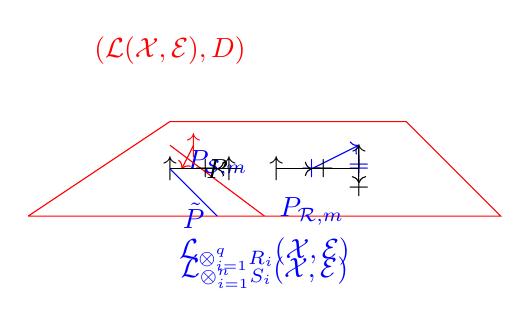
\begin{tikzpicture}[scale=0.6]
    \draw[red] (-5,-2)--(-2,0)--(3,0)--(5,-2)--(-5,-2);
    \node[blue] at (0,-2.8) {$\mathcal{L}_{\otimes_{i=1}^{q}R_i}(\mathcal{X},\mathcal{E})$};
    \node[blue] at (0,-3.2) {$\mathcal{L}_{\otimes_{i=1}^{n}S_i}(\mathcal{X},\mathcal{E})$};
    \node[red] at (-2,1.5) {$(\mathcal{L}(\mathcal{X},\mathcal{E}),D)$};
    \node at (-2,-1) {$\uparrow$};
    \draw[blue] (-2,-1)--(-1,-2);
    \node[blue] at (-1.5,-2) {$\tilde{P}$};
    \node[blue] at (2,-1) {$+$};
    \node[blue] at (1,-1) {$+$};
    \node[blue] at (1,-1.9) {$P_{\mathcal{R},m}$};
    \draw[blue,->] (1,-1)--(2,-0.5);
    \node[blue] at (2,-0.9) {$+$};
    \node[blue] at (-1,-0.9) {$P_{\mathcal{S},m}$};
    \draw[red] (0,-2)--(-2,-0.5);
    \node[red] at (-1.5,-0.5) {$\uparrow$};
    \draw[red,->] (-1.5,-0.5)--(-1.75,-1);
    \draw[black] (-2,-1)--(-0.5,-1);
    \node[black] at (-0.75,-1) {$\uparrow$};
    \draw[black,->] (-0.75,-1)--(-1,-1);
    \node[black] at (-1.25,-1) {$+$};
    \draw[black] (2,-1)--(0.5,-1);
    \node[black] at (0.25,-1) {$\uparrow$};
    \draw[black,->] (0.25,-1)--(1,-1);
    \node[black] at (1.25,-1) {$+$};
    \node[black] at (-1,-1) {$P$};
    \draw[black] (2,-0.5)--(2,-1);
    \node[black] at (2,-0.75) {$\uparrow$};
    \draw[black,->] (2,-0.75)--(2,-1.3);
    \node[black] at (2,-1.4) {$+$};
    \end{tikzpicture}

\end{document}